\chapter{Données expérimentales disponibles} 

\lettrine{C}{e} chapitre explique l'expérimentation qui a été menée en 2017 sur deux vergers dans la commune de Saint-Paul (à la Réunion). 
On décrira le dispositif de l'expérimentation et les données qui en ont étés acquises.
Le but de cette expérimentation était de déterminer quel est l'impact de la modalité de couverture du sol dans le degré d'infestation d'un verger.


\section{Dispositif expérimental et suivis}

Le verger expérimental (que l'on apellera aussi parcelle par la suite) n\textdegree1 a une superficie de 0.33 hectares et est séparé en trois sous-parcelles comprenant chacune trente arbres [À CHECKER].
Sur chacune des trois sous-parcelle, une modalité de couverture du sol différente est mise en place.
Sur un côté il y avait un enherbement entretenu de sorte qu'il reste ras, la modalité \emph{enherbement ras (ER)} fera référence à ce traitement dans la suite du document.
La sous-parcelle du milieu fut baché, afin que les cécidomyies ne puissent ni entrer dans le sol ni en sortir ; cette modalité correspond au \emph{paillage synthétique (PS)}. 
La dernière partie fut laissée telle quelle, sans entretien particulier, donnant ainsi un \emph{enherbement haut (EH)}.
À noter qu'à côté de ce verger, il y en avait un autre qui a probablement pu servir de source d'infestation exogène au verger expérimental.
Tout cela est schématisé sur la figure~\ref{fig:exp}.
Le dispositif sur la parcelle n\textdegree2, comprenant également ces trois modalités de couverture de sol, est décrit dans l'annexe~\ref{chap:bloc2}.
\begin{figure}[ht]
 \centering
 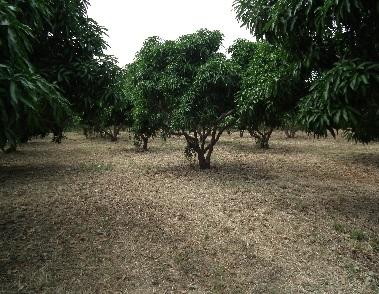
\includegraphics{photos/er.jpg}
 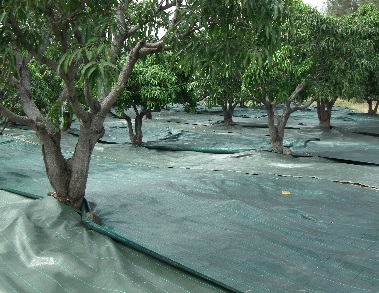
\includegraphics{photos/ps.jpg}
 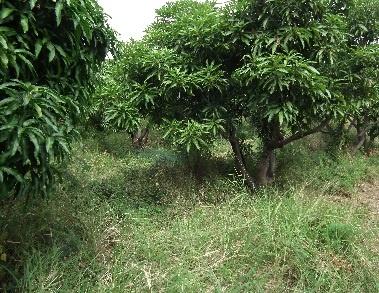
\includegraphics{photos/eh.jpg}
 
 \vspace*{0.5cm}
 
 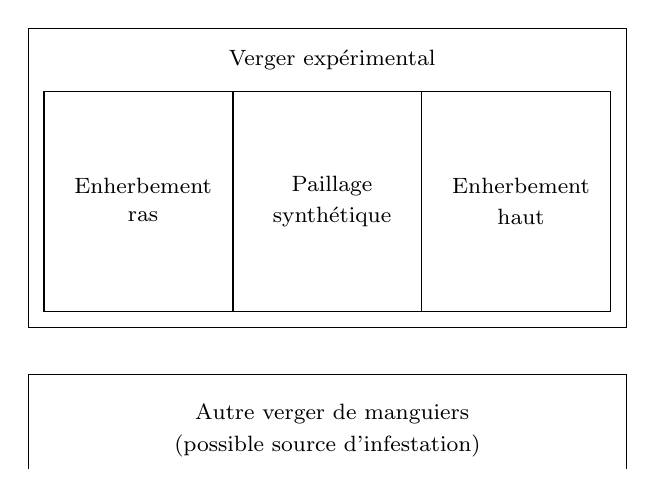
\begin{tikzpicture}[scale = 0.4]
  \draw (0,5) rectangle (18, 12);
  \draw (6, 5) -- (6, 12);
  \draw (12, 5) -- (12, 12);
  \draw (-0.5, 0) -- (-0.5, 3) ;
  \draw (-0.5, 3) -- (18.5, 3) ;
  \draw (18.5, 3) -- (18.5, 0);
  \draw (9, 1.75) node{\text{ \footnotesize Autre verger de manguiers}};
  \draw (9, 0.75) node{\text{\footnotesize (possible source d'infestation)}};
  \draw (9, 9) node{\text{ \footnotesize Paillage}};
  \draw (9, 8) node{\text{ \footnotesize synthétique}};
  \draw (3, 9) node{\text{ \footnotesize Enherbement}};
  \draw (3, 8) node{\text{ \footnotesize ras}};
  \draw (15, 9) node{\text{ \footnotesize Enherbement}};
  \draw (15, 8) node{\text{ \footnotesize haut}};
  \draw (-0.5, 4.5) rectangle (18.5, 14);
  \draw (9, 13) node{\text{ \footnotesize Verger expérimental }};
 \end{tikzpicture}
 \caption{Description du dispositif expérimental de la parcelle n\textdegree1. 
 En haut, photographie des trois modalités de couverture du sol : enherbement ras, paillage synthétique et enherbement haut.
 En bas, schéma du dispositif expérimental et de la configuration des sous-parcelles.  Le verger sur lequel ont été testées les trois modalités de couvertures du sol était situé à côté d'un autre verger.}
 \label{fig:exp}
\end{figure}

Sur ces deux vergers expérimentaux, deux types d'observations furent effectués entre juin et octobre 2017. 
Le premier porte sur les inflorescences. 
Huit unités de croissance furent sélectionnées sur chacun des vingt-cinq arbres échantillonés aléatoirement dans chacune des trois sous-parcelles.
Et c'est ainsi qu'entre le 26 juin et le 3 octobre 2017 furent notés les dates de débourrement des inflorescences présentes sur les deux cents unités de croissance suivies.
À partir du 6 septembre furent aussi notées les dates de mort des inflorescences.
Les relevés ont étés effectués deux fois par semaine.
Les données de ce relevé seront rassemblées en un jeu de données que l'on nommera \emph{dataset 1}.

La seconde catégorie d'observations porte sur la capture des larves de cécidomyies des fleurs.
Dans chacune des trois sous-parcelles, dix arbres furent sélectionnés. 
Sous chacun de ces arbres furent placés deux pièges en dessous des inflorescences présentes.
Les pièges sont des bidons plastiques carrés de douze centimètres de côté remplis d'eau.
À noter que les pièges furent déplacés au cours du temps pour qu'ils soient toujours en-dessous d'inflorescences.
Et c'est ainsi qu'entre le 18 juillet et le 6 octobre 2017 furent notés le nombre de larves piégées, le nombre d'inflorescences vivantes au-dessus du piège et le nombre d'inflorescences vivantes dans l'arbre.
Les relevés ont étés effectués deux fois par semaine.
Les données de ce relevé seront rassemblées en un jeu de données que l'on nommera \emph{dataset 2}.

\section{Données}

Après mise en forme des données\footnote{Les scripts et les données utilisés sont disponibles à l'adresse \url{https://github.com/bastienreyne/cecidomyie}}, on peut extraire les dynamiques qui nous intéressent.
Il faut cependant noter que les deux jeux de données n'ont pas la même échelle (200 unités de croissance contre 10 arbres) et ont été acquis sur des sous-échantillons d'arbres différents.
On choisira de tout mettre à l'échelle de la sous-parcelle.

\subsection{Inflorescences vivantes}

On peut extraire les dynamiques d'inflorescences vivantes grâce aux deux jeux de données : elles seront notées $I^1_t$ pour le \emph{dataset 1} et $I^2_t$ pour le \emph{dataset 2}.
Pour le \emph{dataset 2}, on possède le nombre d'inflorescences vivantes dans les arbres suivis aux différentes dates; il suffit alors de mettre à l'échelle de la sous-parcelle comme suit :
\[
I_{t}^{2} = \frac{N}{n}\sum_{k=1}^{n} I^{2}_{k, t},
\]
avec $N$ représentant le nombre d'arbre dans la sous-parcelle, $n$ le nombre d'arbre suivis et $I^{2}_{k, t}$ le nombre d'inflorescences sur l'arbre $k$ à la date $t$.
À noter que l'on choisira un pas de temps journalier, le nombre d'inflorescences vivantes entre deux relevés effectif est alors le résultat d'une interpolation linéaire entre lesdits relevés.

Pour le \emph{dataset 1}, on possède le nombre de débourrements journalier $B_t$ et le nombre de morts journalier $D_t$.
Le nombre d'inflorescences vivantes au jour $t$ s'écrit alors
\[
I_t^1 = \alpha\left( \sum_{j=1}^{t} B_j - \sum_{j=1}^{t} D_j \right),
\]
où $\alpha$ représente le coefficient de mise à l'échelle pour passer de deux cents unités de croissance à la sous-parcelle.
Il faut cependant apporter une correction à cette dynamique.
En effet, l'observation des inflorescences mortes n'a été faite qu'à partir du 6 septembre.
De ce fait, sur ce jeu de données la distinction entre inflorescences vivantes et mortes n'est possible qu'à partir du 6 septembre.
Il en résulte une forte diminution du nombre d'inflorescences entre le 5 et le 6 septembre (voir figure~\ref{fig:inflos}).
Cet écart correspond au nombre de mort cumulé jusqu'au 6 septembre, et qu'il faut donc répartir sur la période concernée.
N'ayant aucune indication de comment la répartir, on utilisera la dynamique d'inflorescences vivantes du \emph{dataset 2} afin que la dynamique du \emph{dataset 1} y ressemble le plus possible --- et on en profitera au passage pour estimer le coefficient de mise à l'échelle $\alpha$.
Plus précisément, on attribuera un poids (à calibrer numériquement) pour tous les jours entre le jour 1 et le 5 septembre, et le nombre de morts chaque jour sera donné par la formule
\[
D_{t}^{c} = \frac{p_t\times m}{\sum_{j}p_j},
\]
où $D_{t}^{c}$ désigne le nombre de mort à la date $t$, $m$ le nombre de mort observés au 6 septembre et $p_t$ le poids assigné au jour $t$. 
Les poids $p_t$ et le coefficient de mise à l'échelle $\alpha$ seront déterminés numériquement afin de résoudre le problème
\[
\arg\min_{\alpha, p_t} \sum_{t}\left|I^{2}_{t} - I_{t}^{1, c}\right|, 
\]
où $I_{t}^{1, c}$ représente les inflorescences vivantes du \emph{dataset 1} mises à l'échelle et corrigées ; cette dynamique est determinée par la formule
\[
I_{t}^{1, c} = \begin{cases}
                I_t^1 - D_t^{c} & \text{si } t \leq 6 \text{ septembre},\\
                I_t^1 & \text{sinon}.
               \end{cases}
\]
Les différentes dynamiques d'inflorescences sont visibles sur la figure~\ref{fig:inflos}.
On remarque des dynamiques très différentes pour la modalité «enherbement haut» selon le \emph{dataset} considéré, et ce même après correction de la dynamique issue du \emph{dataset 1}.
On peut expliquer ce phénomène par la grande variabilité de la phénologie chez le manguier ; ainsi des échantillonages différents peuvent produire des dynamiques très différentes.
Les deux autres modalités ont en revanche des dynamiques similaires (après correction).
\begin{figure}[ht]
\centering
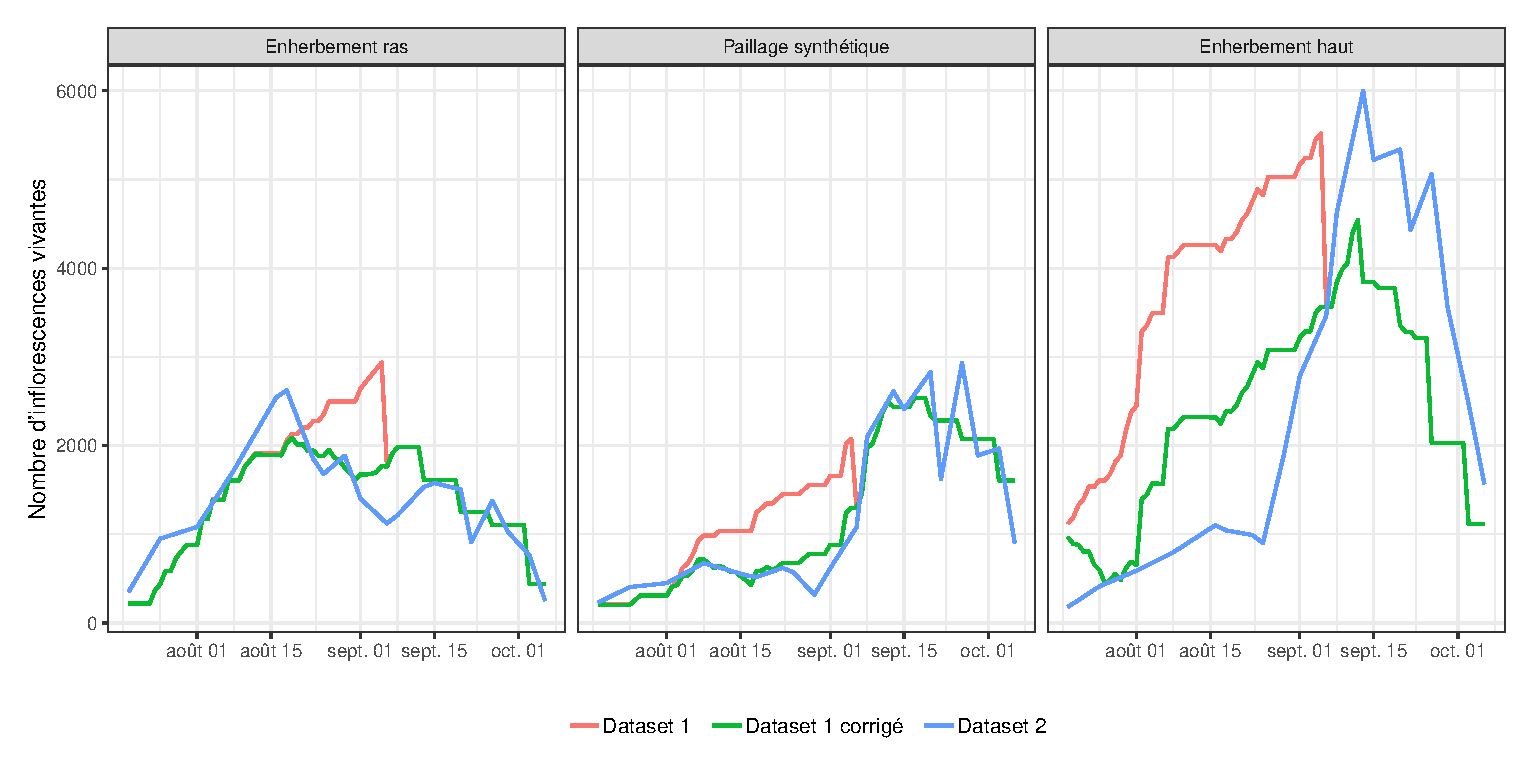
\epsfig{file = r/inflos_vivantes.eps, scale = 0.59}
\caption{Comparaison des différentes dynamiques d'inflorescences vivantes du verger n\textdegree1 en fonction du \emph{dataset} utilisé.}
\label{fig:inflos}
\end{figure}

On fera le choix de privilégier, à chaque fois que cela s'avèrera possible, les dynamiques issues du \emph{dataset 2}.
Ce choix découle du fait que ce sont les dynamiques associées aux dynamiques de larves.


\subsection{Larves}

Le \emph{dataset 2} permet aussi d'extraire la dynamique de larves, à partir des larves piégées.
En effet, on connait le nombre de larves par piège, le nombre d'inflorescences vivantes situées au-dessus des pièges et le nombre d'inflorescences vivantes dans les arbres suivis.
De là, on peut estimer le nombre de larves qui s'éjecte des inflorescences à l'échelle d'un arbre, puis à l'échelle de la sous-parcelle.
Il y a cependant ici une subtilité : le relevé des pièges n'est pas quotidien, il faut donc répartir le nombre de larves piégées entre deux relevés effectifs sur la période entre lesdits relevés.
La dynamiques de larves peut donc s'obtenir en utilisant la formule 
\[
L_t = \frac{N}{n}\left(\sum_{k = 1}^n L_{t}^{k} \times \frac{I_{k, t}^{2}}{I_{k, t}^{2, p}} \right),
\]
où $N$ représente le nombre d'arbre dans la sous-parcelle, $n$ le nombre d'arbre suivis, $I^{2}_{k, t}$ le nombre d'inflorescences sur l'arbre $k$ à la date $t$, $I^{2, p}_{k, t}$ le nombre d'inflorescences au-dessus des pièges dans l'arbre $k$ à la date $t$ et on définit $L_t^k$, le nombre de larves dans les pièges de l’arbre $k$ à la date $t$, par
\[
L_t^k = \frac{L_{k, t}^j}{t^j - t^{j-1}},
\]
avec $t^j$  le nombre de jours entre la première observation et le $j^{\text{ème}}$ relevé et $L_{k, t}^j$ le nombre de larves dans les pièges de l'arbre $k$ au $j^{\text{ème}}$ relevé.
Les différentes dynamiques de larves sont visibles sur la figure~\ref{fig:larves}.
\begin{figure}[ht]
\centering
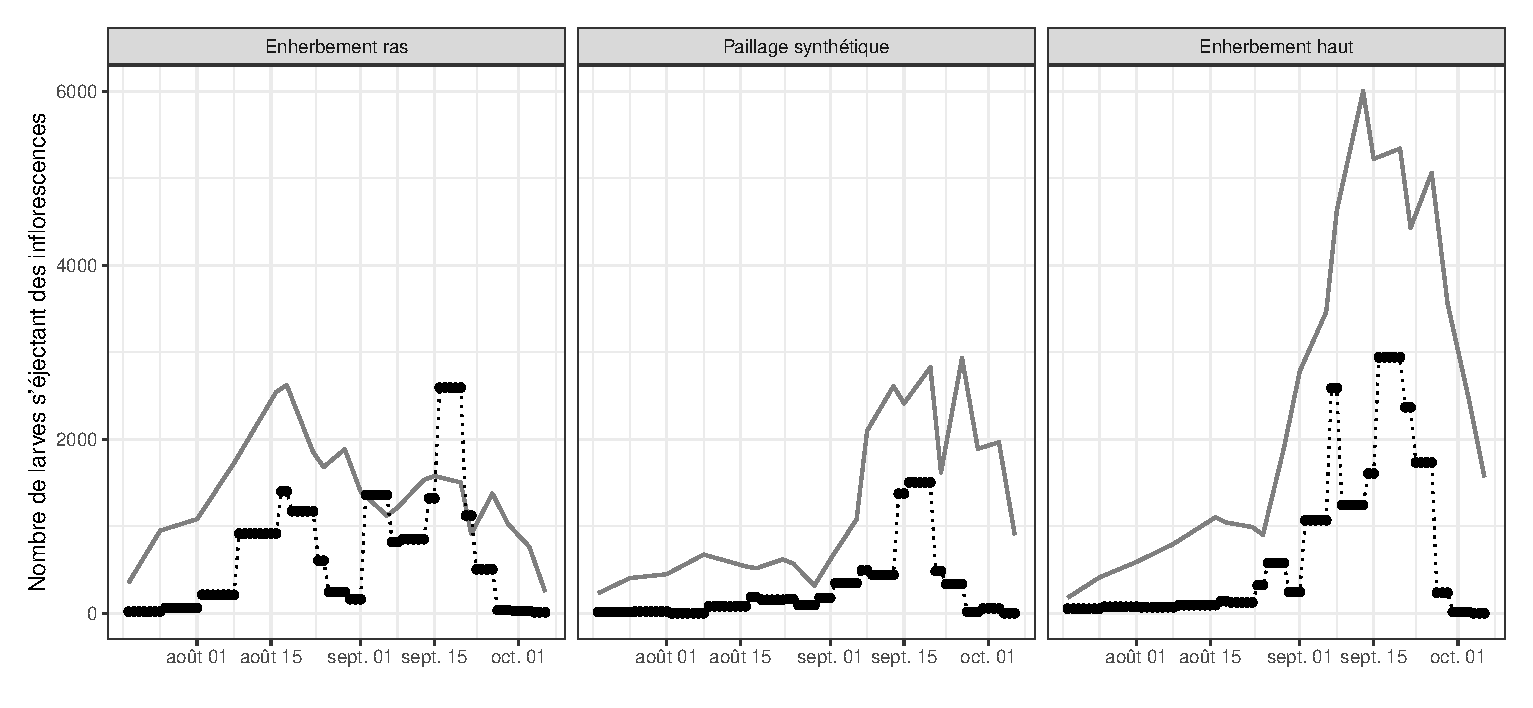
\epsfig{file = r/larves.eps, scale = 0.59}
\caption{Dynamiques de larves s'éjectant des inflorescences des manguiers chaque jour dans le verger n\textdegree1 pour chacune des trois sous-parcelles. En gris sont visibles les dynamiques d'inflorescences vivantes (issues du \emph{dataset 2}, $I^2_t$).}
\label{fig:larves}
\end{figure}

Les dynamiques pour le verger n\textdegree2 sont visibles dans l'annexe~\ref{chap:bloc2}.
